\documentclass[conference]{IEEEtran}

\usepackage{epsfig}
\usepackage{fancyvrb}
\usepackage{url}

\DefineVerbatimEnvironment%
  {code}{Verbatim}{numbers=left,numbersep=3pt,frame=lines,%
                   xleftmargin=7pt,fontsize=\footnotesize}




\begin{document}


\title{A Component-Based Sensor Network for \\ Environmental Monitoring}

\author{\authorblockN{A. Puder, T. Johnson, K. Sales, M. de Sales}
\authorblockA{San Francisco State University \\
Computer Science Department \\
1600 Holloway Avenue \\
San Francisco, CA 94132 \\
EMail: \{arno$\mid$tlj$\mid$klebers$\mid$msales\}@sfsu.edu}
\and
\authorblockN{D. Robinson}
\authorblockA{San Francisco State University \\
Romberg Tiburon Center \\
3150 Paradise Drive \\
Tiburon, CA 94920 \\
EMail: dhr@sfsu.edu}}


\maketitle
\begin{abstract}
  Abstract.
\end{abstract}


\section{Introduction}

Mention the nature of our sensor network: highly specialized sensors,
sparse topology, remote locations, long range communication.
\cite{roemer:2004}

---

Environmental monitoring depends on the reliable collection of
measurements from remotely deployed sensors and the rapid transfer of
those measurements to data centers where processing and analysis may
take place. Typically, sensors are deployed in out-of-the-way
locations, where physical access is limited and connections for
telemetry are poor or nonexistent. Maintaining the data stream from
these sensors places demands on human resources, requiring site visits
to service the sensors and to download data stored on internal memory.
Consequently, there is a lag of days to months between the time the
sensors perform the measurements and the time the measurements become
available. Advances in battery life and anti-fouling technology have
extended service cycles for field sensors, with the unwanted result of
further delaying access to monitoring data.  In addition, the
dependence on field site visits to alter of sensor characteristics, 
such as sampling rate, prevents adjustment in monitoring strategy in
response to rapidly developing events (e.g. oil spills, harmful algal
blooms).

To address these problems of data collection from remote
sensors, we propose to develop an automated end-to-end system based on
proven technology. It provides means to program and interrogate
sensors at the remote field locations and to transmit collected
measurements over long distances to data collections centers, where the
data is rapidly processed, archived, and made available to potential
users in near real-time.

\section{Background}
\label{SEC_BACKGROUND}

Researchers in the geosciences rely on sensor data collected by highly
specialized sensors such as the Seabird or YSI. These sensors are
usually deployed in remote locations that not only make their
maintenance difficult, but also access to their measurements.
Typically, the sensors are autonomous in the sense that they can run
for a certain time on battery power and store the measurement data in
internal memory. Only when the sensors are serviced, the measurement
data, which was collected since the last servicing, is uploaded to a 
portable storage device. From there, the data can be uploaded to
server. Notice that this manual procedure to retrieve sensor data is not only
error prone, but also results are in a serious time lag between the time
the sensor performs the measurement and when it becomes available for
further processing. For many applications, however, it would be beneficial to
have near-realtime access to the sensor measurement. In this way, being able 
to access data when they become available on the sensor device would also
reduce the maintenance overhead.

---

The YSI 6600EDS V2 Sonde \cite{Sonde01} is a water quality monitoring device that
gathers water quality data, and operates in fresh, sea, or polluted
water. Some of the measurements that the YSI is capable of are
conductivity, temperature, chloride, ammonium, nitrate, turbidity, and
chlorophyll.  It is under 55 cm in length, 8.9 cm in diameter, and
weighs approximately 3.18 kg. It operates at temperatures between -5
to +50 deg C and at depths up to 200 meters.  It uses 8 C-size
Alkaline Batteries or External 12 VDC. Battery life can last up to 75
days depending on sensor configuration. The Sonde's bulkhead contains
multiple pin connectors to support sensor probes for measuring the
following:

\begin{table}[h]
\caption{\label{TAB_SONDE_MEASUREMENTS} YSI Sonde measurements.}
\centering
\begin{tabular}{|l||l|}
\hline
\multicolumn{1}{|c||}{\textbf{Name}} &
\multicolumn{1}{c|}{\textbf{Description}} \\ \hline \hline
\texttt{Date}    & Year/Month/Day. \\ \hline
\texttt{Time}    & Hour:Minute:Second. \\ \hline
\texttt{Temp}    & Temperature in degrees Celcius. \\ \hline
\texttt{SpCond}  & Specific Description in microSiemens
                   per centimeter. \\ \hline
\texttt{Cond}    & Conductivity in microSiemens per centimeter. \\ \hline
\texttt{Resist}  & Resistivity in Ohms $*$ centimeter. \\ \hline
\texttt{Sal}     & Salinity in parts per thousand. \\ \hline
\texttt{Press}   & Pressure in pounds per square inch relative. \\ \hline
\texttt{Depth}   & Water column in meters. \\ \hline
\texttt{pH}      & pH in standard units. \\ \hline
\texttt{phmV}    & millivolts associated with the pH reading. \\ \hline
\texttt{ODOSat}  & Dissolved oxygen in \% air saturation. \\ \hline
\texttt{ODOConc} & Dissolved oxygen in mg/L. \\ \hline
\texttt{Turbid}  & Turbidity in nephelometric turbidity units. \\ \hline
\texttt{Battery} & Total Volts remaining in batteries.  \\ \hline
\end{tabular}
\end{table}


Each probe may have multiple sensors.  A computer can interface with
the Sonde via RS-232C or SDI-12. The Sonde can be configured to
collect data samples in discrete or unnattended mode.  Discrete mode
is normally performed while a technician manages the Sonde during the
sampling process. In this mode the Sonde is usually connected via 650
MDS Display/Logger or a serial cable connected to a PC.  The sampling
frequency is usually set to a high frequency in this mode.  Unattended
mode is performed usually when the Sonde is deployed offshore or in a
remote body of water.  The sampling frequency is usually set for a
longer period of time (i.e. 5 - 15 min). The Sonde is configured via a
set of menus that can be accessed through a terminal session over
RS232. Through these menus, the Sonde can be configured to start
logging data to an internal file.  To view the data as it's being
captured, the option to show live data is chosen and the data can then
seen via a serial terminal session at each interval.

---

Start with some related work. Who else has done an OSGi-based
infrastructure for sensor networks? Kleber: I believe you have a few
references. This section should be a combination of a use case (using
the RTC and their YSI sonde as an example) and a requirements
analysis: requirements such as remote management and monitoring
capabilities, time-delayed communication, etc. In this section should
be no mentioning of DSP. Length: 1 page.

\section{Data Sensor Platform}

Should describe DSP architecture. Only mention OSGi in last subsection
and explain that components can be mapped to bundles. Currently no
distinction between Platform and Framework. Necessary?


\subsection{Architecture}

Our architecture is based on a micro-kernel approach. The core
functionality is limited to a minimum and all extra services are built
as plug-and-play modules on top of the micro-kernel. With the help of
this approach we can keep the basic infrastructure compact while
allowing customization via special-purpose modules. In our terminology
we call the basic foundation the \emph{Data Sensor Platform}
(DSP). The scope of the DSP is one address space of an execution
platform. A sensor network is built from several DSPs that are linked
with each other.

Figure \ref{FIG_DSP} depicts the basic architecture of the
DSP. We refer to the plug-and-play modules as DSP Components. DSP
Components are self-contained modules that can be added and removed to
a DSP installation at runtime. The basic communication paradigm within
a DSP is a message. DSP Components can exchange messages of different
types. We distinguish between Data Producers (DP) and Data Consumers
(DP) within the scope of a DSP. DP and DC can be seen as roles that a
DSP Component may have. It is possible for a DSP Component to act in
the role of DC and DP at the same time.


\begin{figure}
\centering
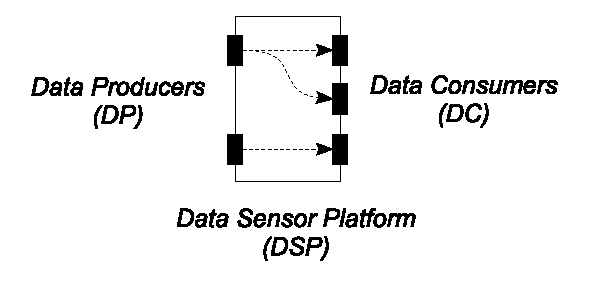
\epsfig{file=dsp, width=7cm}
\caption{\label{FIG_DSP} Data Sensor Platform (DSP).}
\end{figure}

The DSP is responsible for routing messages between DPs and DCs. It is
important to note that this routing only happens withing a
DSP. Following the paradigm of a micro-kernel approach, the DSP has no
notion of remote communication or sensor-specific details. All this
knowledge is embodied in DSP Components.

\subsection{DSP Components}

A DSP Component encapsulates a particular functionality. We
distinguish between those components that produce data (DP) and those
that consume data (DC). An example for a DSP Component acting in the
role of a DP is a sensor module. The sensor module reads data from the
physical sensor and converts the data into a message that is forwarded
to the DSP. Because this module generates data with respect to the
DSP, it is a data producer. An example for a data consumer is a
converter module that converts the internal, DSP-specific data format,
suitable for consumption by external applications. One such common
format used in the domain of environmental monitoring is OpenDAP
\cite{opendap01}. Since the converter module accepts messages from the DSP, it
acts in the role of a data consumer. Finally, a DSP Component
implementing persistency is an example of a module that acts in the
roles of both data producer and consumer. It accepts messages from the
DSP and stores them in a database. At a later time, it may act as a
data producer by resending previously stored messages.

All DSP Components need to implement the following Java interface:

\begin{code}
interface DSPComponent
{
   public String getComponentType();
   public void initComponent(...);
   public void startComponent();
   public void stopComponent();
   public void deliver(DSPMessage msg);
   public Message deliverWithReply(DSPMessage msg);
   // ...
}
\end{code}

By implementing the above Java interface, the resuling code
effectively becomes a DSP Component that can be deployed at runtime. A
component is identified by its type. Only one component of a certain
type per DSP is permissible. A string serves as a type identifier that
much be unique across all DSP Components. Upon deploying a DSP
Component, an initialization function is called (line 4). Once a
component is initialized, it may be started (line 5) and stopped (line
6) multiple time (TODO: SHOULDN'T THERE BE ALSO A WAY TO UNDEPLOY A
COMPONENT?) Whenever the DSP wishes to pass a message (that was
generated by some DP), it invokes the \texttt{deliver()} method (ine
7). The message structure will be explained in the following section.

\subsection{Message}

Message passing is the main paradigm for exchanging information within
a DSP. A data producer sends a message with data consumers accept
messages. We make use of XML technologies to define the format of a
message. Specifically, the common header of all messages are defined
via the following XML Schema:

\begin{code}
<xs:schema ...>
  <xs:complexType name="DSPMessage">
    <xs:element name="Header" type="Header"/>
  </xs:complexType>

  <xs:complexType name="Header">
    <xs:sequence>
      <xs:attribute name="messageID"/>
      <xs:attribute name="originatingDP"/>
      <!-- ... -->
    </xs:sequence>
  </xs:complexType>
</xs:schema>
\end{code}

The above XML Schema DSPMessage serves as a base schema for all
messages and itself defines information typically contained in the
header of a protocol data unit. Amongst others, the header contains a
unique message ID (line 8) and the originating DP (line 9). Using the
XML Schema, we use JAXB to generate a type safe API for handling
instances of DSPMessage. Different messages with different payloads
can be defined by creating schemas that derive from DSPMessage. While
inside the DSP all messages are of type DSPMessage, specific DP and DC
can distinguish between different message types based on their runtime
type information.


\subsection{Matcher}

can only route messages within one DSP. No notion of remote DSP
components.

\subsection{OSGi}

OSGi lends itself naturally to implement the DSP.

DSP can be implemented in different ways, but OSGi is a natural match.
DSP Components are mapped to bundles. DSP itself is a bundle.


\section{NetBEAMS}

In the following we present a practical application of the DSP
presented in the previous section. We describe a deployment of the DSP
using sensor owned and operated by the RTC. Our environmental sensor
network is dubbed NetBEAMS (Networked Bay Environmental Assessment
Monitoring System) and allows access to sensor equipment deployed
throughout the San Francisco Bay Area.  Our goal is to address the
problem of data collection from remote sensors by using the DSP to
automatically interrogate sensors at the remote field locations and
transmit the collected measurements over long distances to a backend
server where the data is made available to potential users in near
real-time. This end-to-end system will be a ready-to-use turnkey
solution that is adaptable to a wide variety of sensor types and
requires no programming expertise to operate. Configuration of the
system will be possible when the sensor is deployed in the field via a
web-based interface, eliminating the need for extra site visits by
technicians between service cycles to change systems functionalities
(e.g. sampling rate). We present the NetBEAMS infrastructure by
discussing its hardware and software components.



\subsection{Hardware}

Figure \ref{FIG_NETBEAMS} provides an end-to-end overview of the
NetBEAMS architecture. NetBEAMS is built using multiple installations
of the DSP and by providing special purpose components for the various
tasks. One DSP installation is collocated with each sensor and an
additional DSP is running on the backend server. Because of the remote
locations where each individual sensor is deployed in the field and
the sparse nature of the network, the resulting topology is a tree
structure of depth 1.


\begin{figure*}
\centering
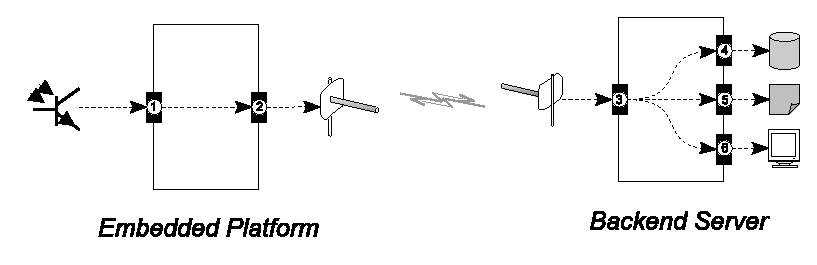
\epsfig{file=netbeams, width=14cm}
\caption{\label{FIG_NETBEAMS} NetBEAMS architecture.}
\end{figure*}

NetBEAMS supports an environmental sensor such as the YSI Sonde,
introduced in Section \ref{SEC_BACKGROUND}. In order to access its
sensor readings, we collocate it with an off-the-shelf embedded
computing platform called Gumstix \cite{gumstix01} (far left in Figure
\ref{FIG_NETBEAMS}). The Gumstix is a single-board computers with 256
Mb of flash and 256 Mb of SDRAM, and running a 600 MHz TI OMAP 3503
processor. Additional features can be added to the motherboard with
expansion cards connected via on-board buses. The motherboards draw
less than 250 mA @4V at 400 MHz and less than 50 mA while idling,
waiting for input.  Gumstix runs Linux 2.6 with the BusyBox utilities,
and uses the OpenEmbedded build environment to provide a complete Linux
environment and a large range of Linux applications. We use the JamVM
\cite{jamvm01} implementation of Sun Microsystem's virtual machine in order to
run the DSP.

The Gumstix connects to the RS232 serial port of the YSI Sonde via via a
null-modem cable.  

We make use of the cellular phone network to establish a communication
link with the backend server. The cellular phone network has the
advantages of reaching well beyond telemetry options such as wireless
networks and being a significantly lower cost solution than satellite
communications. We make use of the Huawei E220. The E220 is a USB
modem that supports HSDPA, UMTS, and EDGE packet data services at maximum
transmission rates of 3.6Mbps, 384kbps, and 236.8kbps respectively.
HSDPA and UMTS operate at 2100MHz while GSM, GPRS, and EDGE operate at
900, 1800, and 1900MHz. The modem connects to the Verdex Pro XM4
motherboard via a mini USB interface (supporting USB 2.0). Linux
kernels since 2.6.20 include support for E220 drivers.  This includes
the linux kernel on the Gumstix which runs 2.6.21.  The Gumstix
communicates with the modem using the PPP protocol and accesses the
cellular network using a data plan from AT\&T.



\subsection{YSI Sonde Component}

Our implementation of the DSP is based on the Open Source
implementation of OSGi called Knopflerfish \cite{knopflerfish01}. Since Sun
Microsystems does not support its JDK for the Gumstix, we use JamVM
\cite{jamvm01} as the Java virtual machine implementation and GNU Classpath
\cite{classpath01} for the runtime libraries. We have implemented various DSP
Components that implement the functionality needed for NetBEAMS. On
the far left of Figure \ref{FIG_NETBEAMS} is the actual sensor; in our
case the aforementioned YSI Sonde. A YSI Sonde data producer (1) is a DSP
component that uses the RS232 standard to read the physical measurements from
the device over a serial port. This component converts the physical measurements 
into a DSP-specific message. The following XML Schema defines the YSI Sonde
specific message that captures all measurement points mentioned in
Table \ref{TAB_SONDE_MEASUREMENTS}:

\begin{code}
<xs:schema ...>
<xs:import schemaLocation="dsp-message.xsd"/>

<xs:element name="SondeDataMessage">
  <xs:complexType>
    <xs:complexContent>
      <xs:extension base="DSPMessage">
        <xs:sequence maxOccurs="unbounded"
                     minOccurs="1">
          <xs:element name="sondeData"
                      type="sondeDataType"/>
        </xs:sequence>
      </xs:extension>
    </xs:complexContent>
  </xs:complexType>
</xs:element>

<xs:complexType name="sondeDataType">
  <xs:sequence>
    <xs:element name="Date" type="xs:date"/>
    <xs:element name="Time" type="xs:time"/>
    <xs:element name="Temp" type="xs:float"/>
    <xs:element name="SpCond" type="xs:float"/>
    <!-- ... -->
  </xs:sequence>
</xs:complexType>
</xs:schema>
\end{code}

The schema is derived from DSPMessage. As a payload it adds an
unbounded sequence of sondeDataType. Each instance of this type
captures one timestamped measure point. The YSI Sonde component can be
configured via special DSP messages that define properties such as the
sampling frequency. These property messages originate from the web
frontend that we will explain in a subsequent section.

\subsection{Remote Communication}

The YSI Sonde component will pass any messages it generates to the
local DSP. Via the matcher configuration these messages are forwarded
to the remote communication component (2). It is the responsibility of
this component to upload the message to its remote peer component
(3). Since we use a data channel of a cellular phone network, the
remote communication component only uploads the buffered data in
certain configurable time intervals. 

\subsection{Web Management}

Web Interface. Management messages are regular
DSPMessages. Asynchronous UI: UI may only build up after next
communication cycle.

\section{Conclusions and Outlook}

The California coastal region is populated by a vast number of
remotely deployed sensors that monitor environmental conditions
ranging from weather to water quality to ocean surface currents.
These sensors are operated by data providers, including resource
management groups, research scientists, municipalities, and state and
federal agencies, who could use near real-time data streams to inform
decision that impact public health, public safety, and the protection
of resources.  In addition, there are efforts underway at the state
and federal level to collate the data collected by the individual data
providers into integrated monitoring networks that will enhance the
distribution of monitoring data to public, private, and federal users
groups.  Success of these efforts, whether small scale or a large
integrated network, depends on the first step in the data management
process: reliably obtaining data in near real-time from remotely
located sensors.  This step can be the weak link in the data
management pathway when telemetry options are unreliable.  The
availability of a plug-and-play computing platform designed to
communicate with a variety of sensor types and to provide data
telemetry to distant brick and mortar data centers would stabilize
data streams with poor telemetry and allowing expansion of sensor
coverage into regions not presently served.  The low power consumption
and low cost of these units would be particularly beneficial for
applications with long service cycles and for data providers trying to
maintain data streams on a limited budget.

\bibliography{lit}
\bibliographystyle{plain}


\end{document}
